
\documentclass[tikz,border=5pt]{standalone}

% Core packages
\usepackage{amsmath,amssymb}
\usepackage{tikz}
\usepackage{tikz-cd}
\usepackage{pgfplots}
\usepackage{multicol}
\usepackage{xcolor}
\usepackage{caption}
\usepackage{float}
\usepackage{kotex}

% TikZ / PGF configuration
\usetikzlibrary{
  arrows.meta,
  calc,
  positioning,
  shapes.geometric,
  shapes.symbols,
  fit,
  backgrounds,
  patterns,
  matrix,
  intersections,
  decorations.pathmorphing,
  decorations.markings,
  angles,
  quotes
}
\pgfplotsset{compat=1.18}

% Reusable TikZ styles
\tikzset{
  >=stealth,
  line cap=round,
  line join=round,
  every picture/.style={line width=0.9pt},
  box/.style={draw, rounded corners, minimum width=2.8cm, minimum height=1.2cm, align=center},
  circlebox/.style={draw, circle, minimum size=1cm, align=center},
  arrow/.style={->, thick},
  dashedarrow/.style={->, thick, dashed},
  point/.style={circle, fill, inner sep=1.2pt},
  gridhelp/.style={help lines, gray!35},
  highlight/.style={fill=blue!10, draw=blue!60!black},
  3D/.style={
    x={(-0.60cm,-0.42cm)},
    y={(0.78cm,0cm)},
    z={(0cm,0.78cm)}
  }
}


\begin{document}

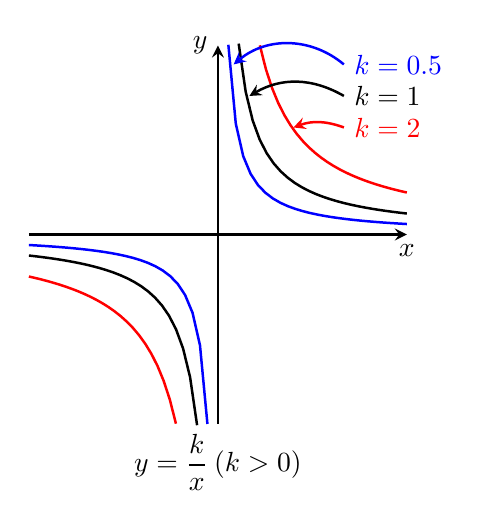
\begin{tikzpicture}[scale=.8,x=10mm,y=10mm]
  \def\xmin{-3}
  \def\xmax{3}
  \def\ymin{-3}
  \def\ymax{3}

  \draw[-stealth] (\xmin,0)--(\xmax,0) node[below] {$x$};
	\draw[-stealth] (0,\ymin)--(0,\ymax) node[left] {$y$};
	
  \draw[domain=0.33:3,variable=\x] plot(\x,{1/\x});
	\draw[domain=-3:-0.33,variable=\x] plot(\x,{1/\x});
	
  \draw[domain=0.666:3,variable=\x,color=red] plot(\x,{2/\x});
	\draw[domain=-3:-0.666,variable=\x,color=red] plot(\x,{2/\x});
	
  \draw[domain=0.166:3,variable=\x,color=blue] plot(\x,{0.5/\x});
	\draw[domain=-3:-0.166,variable=\x,color=blue] plot(\x,{0.5/\x});
	
  \draw[-stealth,color=blue] (2,2.7) node[right] {$k=0.5$} to[bend right=40] (0.25,2.7);
	\draw[-stealth] (2,2.2) node[right] {$k=1$} to[bend right=30] (0.5,2.2);
	\draw[-stealth,color=red] (2,1.7) node[right] {$k=2$} to[bend right=20] (1.2,1.7);

  \node[below] at (0,\ymin) {$y=\dfrac{k}{x}\:(k>0)$};
\end{tikzpicture}

\end{document}

